\documentclass{article}
\usepackage{tikz}
\usepackage{amsmath}
\usepackage[paperwidth=36cm,paperheight=28cm,margin=0.3cm]{geometry}
\pagestyle{empty}
\begin{document}
\centering
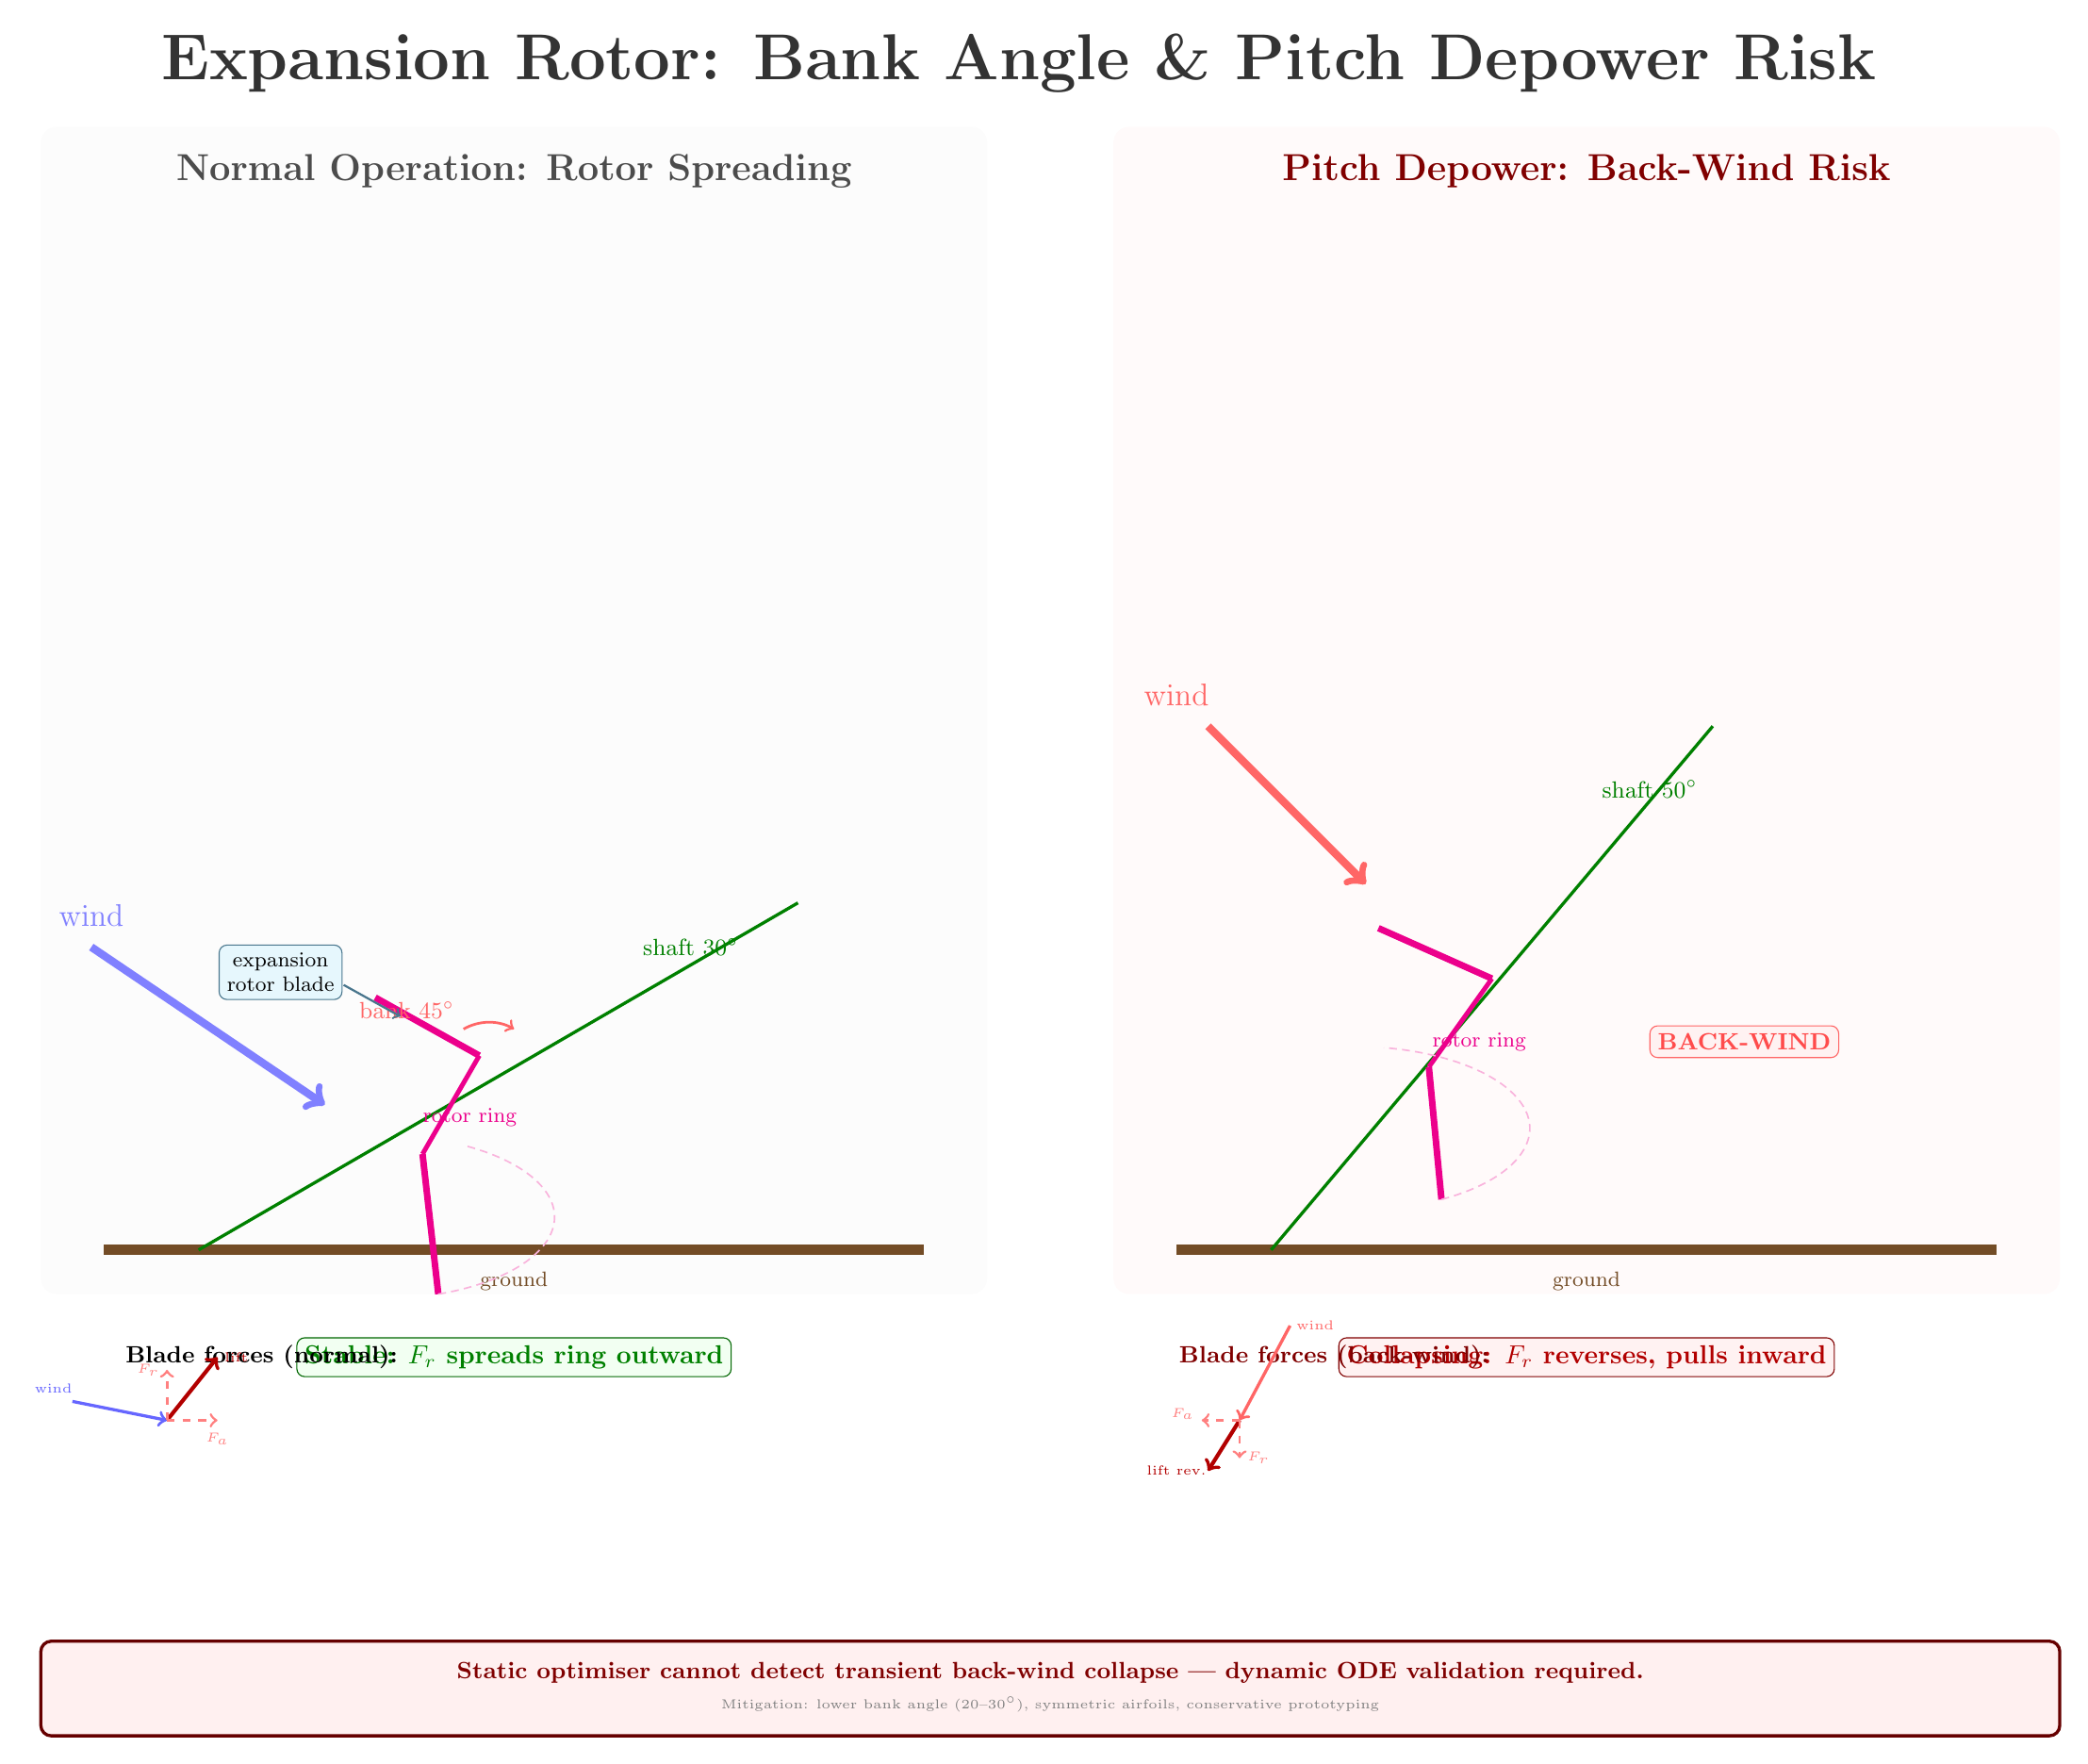
\begin{tikzpicture}[scale=0.85]

% === TITLE ===
\node[font=\bfseries\Huge, black!80] at (15.0,20.5) {Expansion Rotor: Bank Angle \& Pitch Depower Risk};

% ============================================================
% LEFT: Normal operation
% ============================================================
\begin{scope}[shift={(0,1.5)}]
  \fill[black!1, rounded corners=6pt] (-0.5,-0.5) rectangle (14.5,18.0);
  \node[font=\bfseries\Large, black!70] at (7.0,17.3) {Normal Operation: Rotor Spreading};

  % Ground (brown bar)
  \draw[brown!60!black, line width=4pt] (0.5,0.2) -- (13.5,0.2);
  \node[font=\footnotesize, brown!60!black] at (7.0,-0.3) {ground};

  % Shaft axis, 30 degrees, from (2.0,0.2) to (11.5,5.7)
  \draw[green!50!black, line width=1.2pt] (2.0,0.2) -- (11.5,5.7);
  \node[font=\small, green!50!black] at (9.8,5.0) {shaft $30^\circ$};

  % Rotor ring centre at (6.0,2.5) --- ring is perpendicular to shaft
  % Shaft direction: (cos30,sin30)=(0.866,0.5). Perp: (-0.5,0.866) $\\rightarrow$ scaled to length ~0.9
  % Ring endpoints: (6.0-0.45, 2.5-0.78) and (6.0+0.45, 2.5+0.78)
  \draw[magenta, line width=1.8pt] (5.55,1.72) -- (6.45,3.28);
  \node[font=\footnotesize, magenta] at (6.3,2.3) {rotor ring};

  % Upper blade: from top of ring (6.45,3.28), extending up-left
  \draw[magenta, line width=2.5pt] (6.45,3.28) -- (4.8,4.2);
  % Lower blade: from bottom of ring (5.55,1.72), extending down
  \draw[magenta, line width=2.5pt] (5.55,1.72) -- (5.8,-0.5);

  % Bank angle arc
  \draw[->, red!60, line width=1pt] (6.2,3.7) arc (120:60:0.8);
  \node[font=\small, red!60] at (5.3,4.0) {bank $45^\circ$};

  % Callout for expansion blade
  \node[font=\footnotesize, align=center, fill=cyan!10, draw=cyan!50!black, 
        rounded corners=3pt, inner sep=3pt] at (3.3,4.6) {expansion\\rotor blade};
  \draw[->, cyan!50!black, line width=0.8pt] (4.3,4.4) -- (5.2,3.9);

  % Wind arrow
  \draw[->, blue!50, line width=3pt] (0.3,5.0) -- (4.0,2.5);
  \node[font=\large, blue!50] at (0.3,5.5) {wind};

  % Dashed arc for cone sweep
  \draw[magenta!30, line width=0.6pt, densely dashed] (5.8,-0.5) arc (-70:60:2.8 and 1.3);

  % Status
  \node[font=\bfseries, green!50!black, fill=green!5, draw=green!40!black,
        rounded corners=3pt, inner sep=3pt] at (7.0,-1.5) {Stable: $F_r$ spreads ring outward};

  % Force diagram
  \begin{scope}[shift={(1.5,-2.5)}]
    \node[font=\bfseries\small] at (1.5,1.0) {Blade forces (normal):};
    \draw[->, blue!60, line width=1.2pt] (-1.5,0.3) -- (0,0);
    \node[font=\tiny, blue!60] at (-1.8,0.5) {wind};
    \draw[->, red!70!black, line width=1.5pt] (0,0) -- (0.8,1.0);
    \node[font=\tiny, red!70!black] at (1.1,1.0) {lift};
    \draw[->, red!50, line width=1pt, dashed] (0,0) -- (0,0.8);
    \node[font=\tiny, red!50] at (-0.3,0.8) {$F_r$};
    \draw[->, red!50, line width=1pt, dashed] (0,0) -- (0.8,0);
    \node[font=\tiny, red!50] at (0.8,-0.3) {$F_a$};
  \end{scope}
\end{scope}

% ============================================================
% RIGHT: Pitch depower
% ============================================================
\begin{scope}[shift={(17,1.5)}]
  \fill[red!2, rounded corners=6pt] (-0.5,-0.5) rectangle (14.5,18.0);
  \node[font=\bfseries\Large, red!50!black] at (7.0,17.3) {Pitch Depower: Back-Wind Risk};

  \draw[brown!60!black, line width=4pt] (0.5,0.2) -- (13.5,0.2);
  \node[font=\footnotesize, brown!60!black] at (7.0,-0.3) {ground};

  % Shaft at 50 degrees
  \draw[green!50!black, line width=1.2pt] (2.0,0.2) -- (9.0,8.5);
  \node[font=\small, green!50!black] at (8.0,7.5) {shaft $50^\circ$};

  % Rotor ring --- perpendicular to shaft at ~50 degrees
  % Centre at (5.0,3.8)
  \draw[magenta, line width=1.8pt] (4.5,3.1) -- (5.5,4.5);
  \node[font=\footnotesize, magenta] at (5.3,3.5) {rotor ring};

  % Blades --- same mechanical geometry
  \draw[magenta, line width=2.5pt] (5.5,4.5) -- (3.7,5.3);
  \draw[magenta, line width=2.5pt] (4.5,3.1) -- (4.7,1.0);

  % Wind from above
  \draw[->, red!60, line width=3pt] (1.0,8.5) -- (3.5,6.0);
  \node[font=\large, red!60] at (0.5,9.0) {wind};

  \node[font=\bfseries\small, red!70, fill=red!5, draw=red!60,
        rounded corners=3pt, inner sep=3pt] at (9.5,3.5) {BACK-WIND};

  \draw[magenta!30, line width=0.6pt, densely dashed] (4.7,1.0) arc (-60:80:2.8 and 1.3);

  \node[font=\bfseries, red!70!black, fill=red!5, draw=red!50!black,
        rounded corners=3pt, inner sep=3pt] at (7.0,-1.5) {Collapsing: $F_r$ reverses, pulls inward};

  \begin{scope}[shift={(1.5,-2.5)}]
    \node[font=\bfseries\small, red!50!black] at (1.5,1.0) {Blade forces (back-wind):};
    \draw[->, red!60, line width=1.2pt] (0.8,1.5) -- (0,0);
    \node[font=\tiny, red!60] at (1.2,1.5) {wind};
    \draw[->, red!70!black, line width=1.5pt] (0,0) -- (-0.5,-0.8);
    \node[font=\tiny, red!70!black] at (-1.0,-0.8) {lift rev.};
    \draw[->, red!50, line width=1pt, dashed] (0,0) -- (0,-0.6);
    \node[font=\tiny, red!50] at (0.3,-0.6) {$F_r$};
    \draw[->, red!50, line width=1pt, dashed] (0,0) -- (-0.6,0);
    \node[font=\tiny, red!50] at (-0.9,0.1) {$F_a$};
  \end{scope}
\end{scope}

% ============================================================
% BOTTOM BAR
% ============================================================
\fill[red!6, draw=red!40!black, line width=1.2pt, rounded corners=4pt] (-0.5,-6.0) rectangle (31.5,-4.5);
\node[font=\bfseries\small, red!50!black] at (15.5,-5.0) {Static optimiser cannot detect transient back-wind collapse --- dynamic ODE validation required.};
\node[font=\tiny, black!50] at (15.5,-5.5) {Mitigation: lower bank angle (20--30$^\circ$), symmetric airfoils, conservative prototyping};

\end{tikzpicture}
\end{document}
